\documentclass[12pt]{report}
\usepackage[catalan]{babel}
%\usepackage[latin1]{inputenc}   % Permet usar tots els accents i car�ters llatins de forma directa.
\usepackage[utf8]{inputenc}  
\usepackage{enumerate}
\usepackage{amsfonts, amscd, amsmath, amssymb}
\usepackage[pdftex]{graphicx}

\setlength{\textwidth}{16cm}
\setlength{\textheight}{24.5cm}
\setlength{\oddsidemargin}{-0.3cm}
\setlength{\evensidemargin}{0.25cm} \addtolength{\headheight}{\baselineskip}
\addtolength{\topmargin}{-3cm}

\newcommand\Z{\mathbb{Z}}
\newcommand\R{\mathbb{R}}
\newcommand\N{\mathbb{N}}
\newcommand\Q{\mathbb{Q}}
\newcommand\K{\Bbbk}
\newcommand\C{\mathbb{C}}

\newcounter{exctr}
\newenvironment{exemple}
{ \stepcounter{exctr} 
\hspace{0.2cm} 
\textit{Exemple  \arabic{exctr}: }
\it
\begin{quotation}
}{\end{quotation}}

\pagestyle{empty}

\begin{document}

\begin{center}
\textbf{\Large Fonaments i Aplicacions del Processament Digital dels Senyals.\\ 
Control 3. Curs 2011-12}
\end{center}

\vskip 1cm
\noindent
\textbf{P1.} Sigui $X(\omega)$ la transformada de Fourier del senyal $x[n]$ següent:
\[
x[n]=\{ \underline{1}, 0, -1, 2, 3, 0, -3, -2, 1, 0, -1 \}
\]

  Responeu les següents qüestions sense calcular explícitament
  $X(\omega)$. 
  \begin{enumerate}[a)]
  \item Trobeu el valor que pren $X(\omega)$ per $\omega=0$.
  \item Calculeu $\arg X(\omega)$.
  \item Avalueu $\int_{-\pi}^\pi X(\omega)\,d\omega$.
  \end{enumerate}

\vskip 1cm
\noindent
\textbf{P2.}
Considereu el sistema següent, que representa un sistema complet
  de processament digital del senyal analògic:
\begin{center}
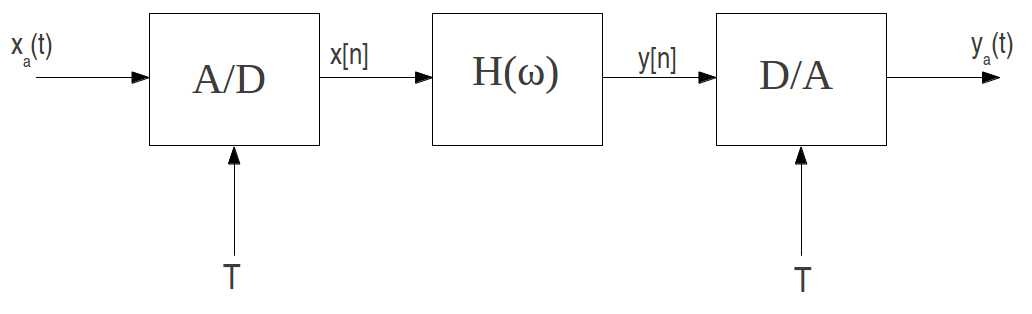
\includegraphics[width=10cm]{adda.png}
\end{center}

On $H(\omega)=\begin{cases} 1 & |\omega| < \frac{\pi}{2} \\ 0 & \text{resta} \end{cases}$.


El senyal d'entrada $x_a(t)$ és un senyal real amb espectre $X_a(\Omega)$ 
de forma triangular, sense components espectrals per damunt dels 5KHz i $X_a(0)=1$.
Es demana:
\begin{enumerate}[a)]
\item Quina és la mínima freqüència de mostreig que evita el problema de l'aliasing?
\item Si consideram una freqüència de mostreig de 15 KHz, dibuixau l'espectre de tots 
els senyals que intervenen en el sistema anterior (incloent els senyals interns dels blocs 
A/D i D/A).
\item Quin és el rang de freqüències de mostreig que garanteix que el sistema global
es comporta com un sistema passa baix ideal?
$\left( H_{eq}(\Omega)=\begin{cases} 1 & |\Omega| < \Omega_c \\ 0 & \text{resta} 
\end{cases}\right)$.
\end{enumerate}




\end{document}
